\documentclass[10pt, conference, compsocconf]{IEEEtran}

\ifCLASSINFOpdf
  \usepackage[pdftex]{graphicx}
  \graphicspath{{./res/}}
  \DeclareGraphicsExtensions{.pdf,.jpeg,.png}
\else  
\fi

\hyphenation{op-tical net-works semi-conduc-tor}


\begin{document}
\title{Methods of Detecting Home Language Shift in Canadian Census Data}

\author{\IEEEauthorblockN{Chris Choy, Kiefer Co, Matthew Fogel, Clarke Garrioch and Katie Martchenko}
\IEEEauthorblockA{Department of Computer Science\\
University of Manitoba\\
Winnipeg, MB, Canada\\
Email: kleung@cs.umanitoba.ca}
}

\maketitle


\begin{abstract}
Canada is a nation composed of a highly diverse language population. This provides a unique opportunity to study the factors causing certain languages and language families to be lost over subsequent generations amongst allophones (people with a mother tongue other than English or French). This paper applies and compares the performance of Decision Tree Induction, Random Forest, and Categorical Naive Bayesian algorithms to census microdata to analyze the influence of various social and economic factors on the probability that allophones adopt official languages as their language spoken at home.

\end{abstract}

\begin{IEEEkeywords}
component; language cohorts; allophones; mother tongue; language persistence

\end{IEEEkeywords}


\IEEEpeerreviewmaketitle



\section{Introduction}
% no \IEEEPARstart
Canada is a nation composed of a highly diverse language population. Immigration and migration has risen both in numbers and as culturally relevant components of modern communities, especially in diverse countries such as Canada.

This provides a unique opportunity to study the rates at which certain languages and language families are lost over subsequent generations as allophones (people with a mother tongue other than English or French) adopt English or French as their primary language. Certain factors such as sex, age, educational status and economic success may prove to be key indicators of how quickly an individual adopts a language other than their mother tongue in everyday life.

A language shift occurs when an allophone adopts an official language as their primary language, i.e. language spoken at home. Several studies have aimed to measure language shift rates through linear regression on various cohorts of the population. Ultimately, it is impossible to ascertain precisely when a language shift occurs, so the insights offered by linear regression are limited in accuracy.

This paper proposes an application of various data mining algorithms and compares their accuracy and speed when used on census data, namely the Random Forest algorithm, the Decision Tree algorithm, and the Categorical Naive Bayesian algorithm.

Some challenges working with census microdata include the fact that the Public Use Microdata Files (PUMF) have been downsampled from the census population size. In order to perform an analysis that would take into account the population distribution, records are needed to be multiplied by a corresponding weight included in the PUMF datasets. Additionally, the PUMF datasets contain over 100 potential features, some of which contain largely invalid/unavailable data. As a result, some level of feature selection is required.

The Canadian census is conducted every five years. As a result, changes that occur between census periods may not be captured at the exact time of their occurrence.


\section{Related Work}
Over the past several years, researchers have come up with multiple approaches to analyze census microdata to determine the rates at which allophones express a language shift. Several authors has focused on identifying whether a  shift towards official languages (English and French) have occurred by determining if the mother tongue is the same as the language spoken at home. This is typically accomplished by performing linear regression.

\subsection{Linear Regression of Language Cohorts}
\subsubsection{Fictitious Cohorts}
Patrick Sabourin and Alain Bélanger use the concept of a 'fictitious cohort', in which groups separated by age or time since immigration are compared across a single census. They define language persistence as the proportion of each cohort that has kept their mother tongue as the language most often spoken at home. The authors analyze language shift using linear regression and polynomial regression. They then construct a survival curve which determines the probability that each subsection of a cohort (such as a specific age group) will undergo a language shift. They make the assumption that the rate of language shift is constant among several censuses.
\cite{dynamics1}

One limitation to this method is that members of a cohort are defined in binary terms as having lost a language if they no longer speak it at home, while this process might occur gradually in real time. Additionally, certain language groups may experience different rates of language shift. \cite{dynamics1}

\subsubsection{Synthetic Cohorts}
Marie T Mora, Daniel J Villa and Alberto Davila use an alternative method known as 'synthetic cohort' analysis on census data in the United States. Their paper aims to better understand the recent dynamic of language loss and intergenerational maintenance of Spanish in the U.S., and compare it to other non-English languages. In other words, exploring the retention or loss of Spanish and other non-English speakers in the U.S., particularly among foreign-born and U.S.-born children with immigrant parents. \cite{spanish1}

The technique for analysis, synthetic cohort analysis, is based on data drawn from 1980, 1990, and 2000 United States Censuses. It creates a temporal representation of a population, over ten-year intervals. The authors track the reported language use of individuals starting at ages 5-7 and ending at ages 15-17 across two United States census. This selection is due to children being able to speak at ages 5-7 and languages tending not to be lost after ages 15-17. \cite{spanish1}

This is in contrast to cross-sectional methods which use data from only one Census period to analyze language shifts. Combining this method with the synthetic cohort, the paper argues that the dynamic in language shift is better predicted, supported by what has been observed in the U.S. \cite{spanish1}

There are still some difficulties with this approach. For example, 1980 and 1990 samples could have emigrations before 1990 and 2000, and from this the “true” cohorts of the foreign-born may not be entirely reflected. \cite{spanish1}

\subsubsection{Limitations of Linear Regression}
As seen above, multiple approaches to analyzing language cohorts temporally run into limitations in how census data is collected. Sampling errors and poorly worded census questions make it difficult to capture whether emigration has occurred between censuses. Even within a census, it is tempting to view language shift within a cohort as binary when this process occurs gradually.

Populations are dynamic, and multiple categorical variables influence whether a language that is the mother tongue is spoken at home. A decision tree can reveal which categorical variables determine whether mother tongue is retained as the language spoken at home.

\subsection{Decision Tree Performance in Other Areas}
\subsubsection{Decision Trees in Student Performance Prediction}
Decision trees have also been compared and applied in other fields. Osmanbegovic and Suljic compared the performance of an implementation of a decision tree algorithm, Naive Bayes algorithm, and a Multilayer Perceptron algorithm in predicting student performance by the prediction accuracy, learning time, and error rate. \cite{performance1}

Osmanbegovic and Suljic used 12 input features such as gender, GPA, and whether or not the student had scholarships, and outputted whether or not the student would pass or fail. The output could also be classified by letter grades, but due to the disparity in the amount of data for each class, was not used. \cite{performance1}

They found that the Naive Bayes algorithm managed to outperform the C4.5 decision tree algorithm implementation, J48, in both prediction accuracy, and error rate. Additionally, it was found that the Naive Bayes algorithm and the decision tree algorithm created prediction models that were both accurate, and user-friendly enough for the stakeholders. \cite{performance1}

\subsubsection{Improvements}
Similarly to Osmanbegovic and Suljic's data, some classes in census data are going to have differing amounts of data, and will affect prediction accuracy. Instead of changing the class groupings to get more equal representation, weights could be added to the training data to account for these differences. In the case of the Canadian Census data, these weights are already added to the data for use.

\subsection{An Alternative Approach to Census Data Mining}
In their paper, Klösgen and May took a different approach to mining census data. Klösgen and May used the United Kingdom's census data, which was only available in an aggregated form. The census data was available aggregated across various wards within the region, along with a detailed set of geographic layers. Thus, Klösgen and May decided to use those wards as the focus of their examination, and propose an application of SubgroupMiner, an advanced subgroup mining system. \cite{census1}

\subsection{An Improved Decision Tree Algorithm}
Hulten, Spencer, and Domingos' CVFDT algorithm improves on the VFDT decision tree learner by accounting for data changing over time. \cite{dtrees1} Their CVFDT algorithm works by maintaining a decision tree with respect to a sliding window of data and grows an alternative subtree to replace an old one if it becomes out of date. This allows for it to learn a similar model to one from the VFDT algorithm but in constant time. \cite{dtrees1}

Applying the algorithm to census data seems like a natural fit, and can be used to improve the performance of any decision tree learners in use. The addition of the time aspect could also be used to improve the accuracy in cases where the data from only one period of time is used, instead of multiple.


\section{Methodology}

\subsection{General Process}
% @TODO expand on this
The general process is as follows:
\begin{enumerate}
	\item Determine when a shift in language occurs
	\item Preprocess the data, converting any continuous values into discrete values
	\item Split the data into training and testing sets
	\item Construct the various classifiers, and evaluate them
\end{enumerate}

Due to the nature of decision trees, all continuous values must be converted into a discrete value. Additionally, differences in datasets may result in the definition of language shift needing to be adjusted.

\subsection{Mining the 2016 Canadian Census}
In addition to the general steps stated above, applying them to the 2016 Canadian Census required further work, namely the additional preprocessing due to the format of the data.

The analysis was performed in Python 3 via Jupyter Notebooks.  
The \textbf{pandas} package was used to import the 2016 PUMF Individuals CSV file as a \textit{DataFrame} and perform manipulations on the \textit{DataFrame}, described in more detail in the data preprocessing section.

Several modules in the \textbf{scikit-learn} package were used for the classification algorithms in question, including the \textit{DecisionTreeClassifier} for classifying based on decision trees, the \textit{RandomForestClassifier} for classifying using random forests, and \textit{CategoricalNB} for classifying using a Naive Bayesian algorithm. More details on these classifiers can be found in their respective sections.

The \textbf{bokeh} package was used to generate a bar chart describing the features with the greatest amount of invalid data and to visualize the ROC AUC scores for the various classifiers. The \textbf{tabulate} package was used to create a table listing feature importances in descending order of importance. The \textbf{graphviz} package was used to visualize decision trees.

\subsubsection{Data Format}
Data was collected from the 2016 Canadian census public use microdata file (PUMF), which contains around 930,421 (or \~2.7\% of the target population) individual, anonymized records, with 123 features. Additionally, there is an individual weight attached to each record, and 16 estimate weights for sampling variability.

While the PUMF did give individual records, some of the data was aggregated to preserve confidentiality (e.g. categories being combined together), and some records had some of their variables changed to 'Not Available' for similar reasons. Furthermore, only the largest of the census metropolitan areas and provinces were covered. 

Since the PUMF data was only a sample of the target population, each record includes an individual weight to indicate how much of the target population that the record represents. In addition to the weights, 31 of the features are drawn from the universe of family, household, and dwelling universes, and the remaining 92 features are from the individual universe.

\subsubsection{Data Preprocessing}
Prior to the execution of any of the classifiers, the PUMF dataset is passed through a single data preprocessing pipeline.  This pipeline achieves two broad objectives, namely pruning uninteresting data and selecting against features containing a high proportion of invalid data.


The feature selection process performed was a mix of manually intuited choices and insights from initial analysis using \textit{scikit-learn}'s decision tree classifier on unprocessed data.  Features which were pruned were both uninformative with regards to the goal of detecting home language shifts and possessed clearly understood reasons for their behaviour.  For example, MTNEN (mother tongue being English) was extremely negatively correlated with the shift metric, as English is the most spoken language in Canada and an unlikely home language to shift away from.  Conversely, LWAEN (language at work being English) and LWAFR (language at work being French), had little to no influence on the shift metric, which was understood to be the consequence of work language rarely being a language other than English or French.  Such features were omitted from the preprocessed version of the dataset.

The initial data analysis also found promising improvements when dropping rows featuring English as a mother tongue.  Removal of these rows lowered the unusable proportion of many features that was thought to provide useful insight, such as AGEIMM (age of immigration) which dropped from 88 to 61 percent unusable.  Although AGEIMM in particular remained unsuitable for the analysis as only a fraction of respondents provided a usable value, a decision was made to remove English mother tongue rows from the dataset with the intention of providing more focused analysis on changes within Canada's non-official language communities, from which shifts to English as a home language were more common than the inverse.

\begin{figure}
  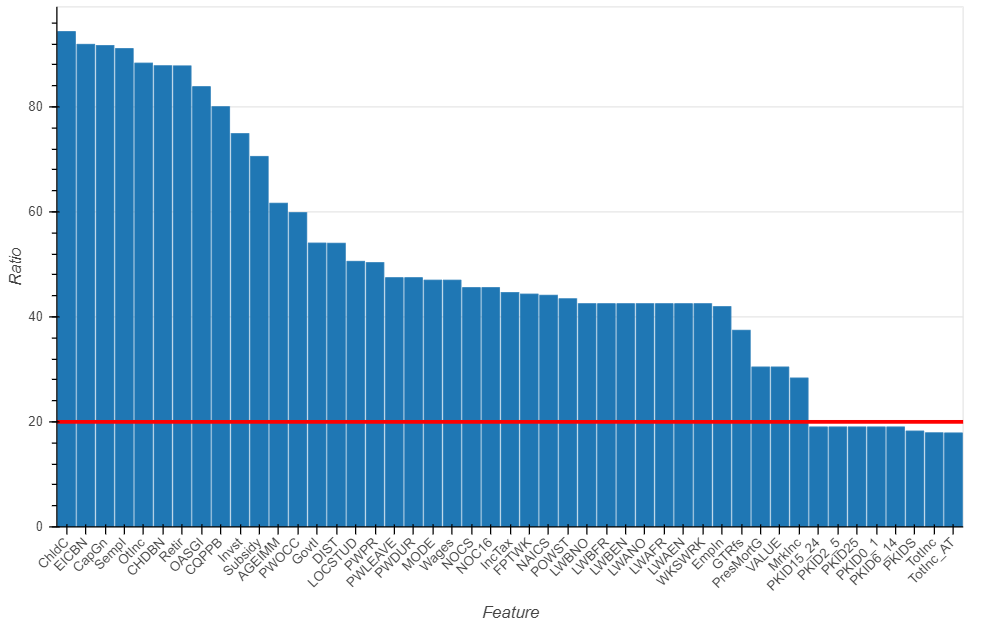
\includegraphics[scale=0.25]{invalid_data_by_feature}
  \centering
  \caption{Invalid data by feature}
  \label{fig:invalid_data}
\end{figure}

The PUMF dataset also contained missing, invalid, or inapplicable values as specified by certain numeric codes (e.g.  88888888) as specified in its accompanying Study Documentation.  The initial preprocessing involved detecting the number of such values in each feature column as a proportion of the total number of entries.  Features which possessed an unusable percentage greater than 20\% were pruned so as to not obscure the analysis by training classifiers on presence of a data feature rather than its content. This was done after the removal of English as a mother tongue rows described earlier. A subset of the feature's invalid data rates can be seen in figure \ref{fig:invalid_data}.

Finally, the data is split into training and testing data sets with 75\% of the data being allocated for training, and the remaining 25\% for testing.

\subsubsection{Imputation}
Since some values in the PUMF data are marked as invalid or unavailable, further preprocessing on the data was required.  As mentioned, data imputation was considered as a remedy for unusable data, but opted against due to the presence of weights attached to each record in the PUMF dataset.  The dataset is meant to balance presenting a representative subset of Canada's demographics while also anonymizing census results which, by Canadian law, are to be withheld from complete public disclosure for 92 years post-response.  As such, each row in the PUMF dataset is a weighted representation of several individuals, listed under the attribute WEIGHT.  Imputation of unusable values, even with the feature's weighted mean as a substitution, was reasoned to be inapplicable without rendering the dataset no longer representative of Canada's demographics.

\subsubsection{Shift Detection}
The process for identifying language shift involves constructing a Boolean feature called \textbf{languageShift}, computed from the MTNNO (mother tongue) and HLANO (home language) attributes.

In the PUMF dataset, both the MTNNO and HLANO features are categorical attributes encoded as a numeric value.  Each feature's encodings are independent and cannot be readily compared, although there exists an intersection between the categories represented within each feature.  Dictionaries for mapping MTNNO and HLANO categories to equivalency classes were manually defined using information outlined in the PUMF Study Documentation file.  These classes include both whole languages such as "Arabic" as well as grouped categories such as "Austro-Asiatic languages".

As the MTNNO categories are less broad and appear to be a superset of the HLANO categories, some categories appear in MTNNO but not HLANO, such as "Uralic" or Korean".  Rather than omitting rows containing these mother tongues, they are categorized under the "All other languages" class.

The value of the languageShift attribute is then defined as the presence of inequivalent class mappings in the MTNNO and HLANO features within a data row.  The reasoning behind this decision is that a difference between mother tongue and home language implies a shift having occurred at some point within an individual's lifetime, with the assumption made being that an individual's mother tongue must at one point have been their home language, possibly only in childhood or even outside of Canada.

If MTNNO can be mapped to HLANO, the languageShift value of a row is false.  If no mapping can be found, the languageShift value will be true.  As with other features in the dataset, the results of the languageShift column are to be interpreted as representative of several individuals.  A row's weight is to be factored into any analysis on or prediction of the languageShift feature. After this preprocessing, the counts of the true class (language shift has occurred) and the false class (language shift has not occurred) are 306,645 and 72,430, respectively. 


\subsection{Decision Tree}
The Decision Tree classifier was build using \textit{scikit-learn}'s implementation, \textit{DecisionTreeClassifier}. To prevent overfitting of the training data, the maximum depth of the decision tree was set to 8 since this is approximately the square root of the number of features being included in the classifier.

The languageShift and WEIGHT attributes are first separated from the dataset to serve as class labels and weights respectively.  MTNNO and HLANO are dropped from the dataset as they are directly involved in the computation of languageShift, for which their effects on a classifier for would be uninteresting.  The remaining attributes in the preprocessed dataset are then to be used as classification features. The features and weights for the training data are then passed into the classifier, with the weights being passed into the \textit{sample weight} parameter of the \textit{fit} function on the decision tree classifier. The class of test samples are predicted using the \textit{predict} function. Finally, the results of the classifier are output in a confusion matrix.

\subsection{Random Forest}

Similarly to the Decision Tree classifier, the Random Forest classifier was constructed using \textit{scikit-learn}'s implementation, \textit{RandomForestClassifier}, using 20 estimators and a controlled random state to maintain similar, repeatable results after multiple runs. As Random Forest classifiers inherently have measures to reduce overfitting of the training data, no maximum depth was specified.

The classifier is trained on the training data set, along with their weights, then evaluated on the testing data set. The predicted class of test samples is determined using the \textit{predict} function by selecting the class with the highest mean probability estimate across all trees in the random forest. The results are also outputted to a confusion matrix.

\subsection{Naive Bayesian}

The Naive Bayesian classifier was built using \textit{scikit-learn}'s \textit{CategoricalNB} - a Naive Bayes classifier for categorical features. This classifier assumes that each feature has its own categorical distribution. The \textit{fit} method was used to train the classifier on the weighted training data. The \textit{predict} method was used to perform classification on the testing data. The results are also outputted to a confusion matrix.

\section{Analytic Evaluation}

\begin{figure}
  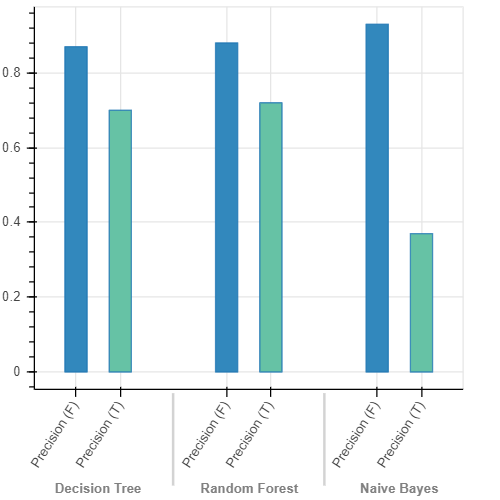
\includegraphics[scale=0.45]{precision}
  \centering
  \caption{Classifier precision values}
  \label{fig:precision}
\end{figure}

\begin{figure}
  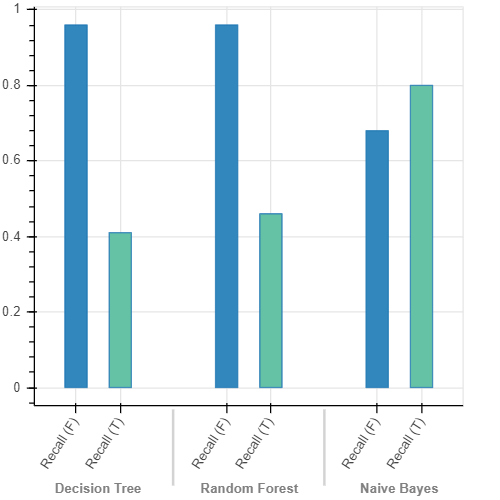
\includegraphics[scale=0.45]{recall}
  \centering
  \caption{Classifier recall values}
  \label{fig:recall}
\end{figure}

\begin{figure}
  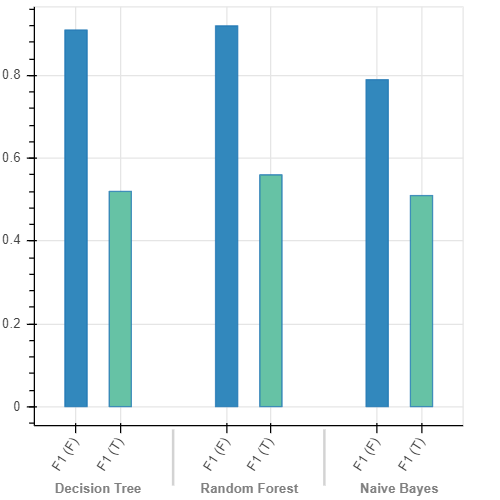
\includegraphics[scale=0.45]{F1}
  \centering
  \caption{Classifier F1 values}
  \label{fig:f1}
\end{figure}

\begin{figure}
  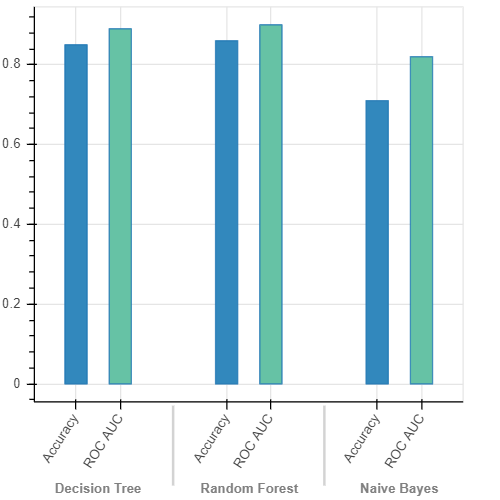
\includegraphics[scale=0.45]{acc_roc}
  \centering
  \caption{Classifier accuracy and ROC AUC values}
  \label{fig:acc_roc}
\end{figure}

To compare the different classifiers, metrics such as precision, recall, F1 score, and AUC ROC scores were used. Additionally, the top 10 feature importances for the Decision Tree classifier, and the Random Forest classifier were examined to further compare the two. The metrics can be seen in figures \ref{fig:decision_tree_metrics}, \ref{fig:random_forest_metrics}, and \ref{fig:naive_bayes_metrics}. Additionally, a graphical representation of the AUC ROC scores can be seen for each of the classifiers in figures \ref{fig:decision_tree_roc}, \ref{fig:random_forest_roc}, and \ref{fig:naive_bayes_roc}. Finally, graphs comparing the classifiers by each of the metrics can be found in figures \ref{fig:precision}, \ref{fig:recall}, \ref{fig:f1}, and \ref{fig:acc_roc}.

Since the target class is highly unbalanced, with roughly 81\% of the data belonging to the false class, accuracy was perhaps not the best metric to use to compare the different models. The other metrics calculated such as F1-scores and AUC ROC scores provide a more accurate assessment for the models.

One noticeable side effect of the imbalanced data was that all of the classifiers tended to perform better by all metrics for the negative class. This is not a surprising fact as the classifiers had trained on more instances of the negative class than the positive class. As seen in figure \ref{fig:recall}, there was one exception to this observation in the recall value for the Naive Bayes classifier.

The ROC AUC scores for the Decision Tree model and Random Forest model are 0.88 and 0.89, respectively. This means they are performing similarly in determining the positive class from the negative class. The ROC AUC score for Naive Bayes is 0.82, 8 percent lower than the two tree-based models. This is a significant difference, and it is reflected in the ROC AUC curve, where a noticeable dip in the curve occurs early on when compared to the tree-based models' curves. From this it can can be determined that the Naive Bayes classifier performs significantly worse at determining the the positive class from the negative class than the tree-based models.

On the other hand, the Decision Tree and Random Forest classifiers performed noticeably better on classifying the negative class. Since the data set was highly imbalanced towards the negative class, it's possible that this resulted in the tree-based classifiers having an overall higher performance than the Naive Bayes classifier.

As shown in figures \ref{fig:precision}, \ref{fig:recall}, \ref{fig:f1}, and \ref{fig:acc_roc}, the Random Forest classifier only provided a slight improvement on the standard Decision Tree classifier. Additionally, the top 10 most important features between the two classifiers are very similar (see figures \ref{fig:decision_tree_importances}, \ref{fig:random_forest_importances}).
% @TODO maybe add another couple of lines here

% @TODO fill in
% observations
% - the decision tree and random forest had very similar feature importances, and precision/recal/etc.
%   - this can also be seen in the ROC AUC's
% - the decision tree and random forest were really good at classifying negative class, not so much the positive class
%   - this could be due to the imbalanced nature of the data; there was a lot more negative examples than positive one
% - the NB classifier had decent recall (with a better recall for the positive class), but a poor precision rate for the positive class
%   - in contrast to the decision tree/random forest where the precision was decent in both classes
%   - kinda similar to that one paper (\cite{performance1}), but NB managed to outperform in recall for all classes and precision
% - f1 score for the Naive Bayes all around worse than the decision tree / random forest
% - ROC AUC for NB was noticeably worse
% - the feature importances for DT/RF are pretty intuitive, with the exception of labour force (didn't look at what that is too much though)

\begin{figure}
  \begin{tabular}{lllll}
                  & precision & recall      & f1-score  & support \\
  \textit{False}  & 0.87      & 0.96        & 0.91      & 76719 \\
  \textit{True}   & 0.70      & 0.41        & 0.52      & 18050 \\
  Total			      &           &             &           & 94769 \\
  Accuracy        & 0.85 \\
  ROC AUC Score	  & 0.89 \\\
  \end{tabular}
  \caption{Decision Tree metrics}
  \label{fig:decision_tree_metrics}
\end{figure}

\begin{figure}
  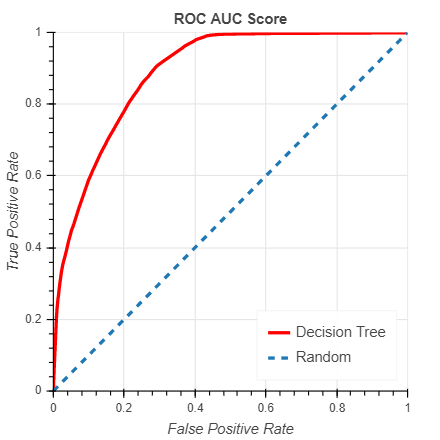
\includegraphics[scale=0.45]{decision_tree_roc}
  \centering
  \caption{Decision Tree ROC AUC curve}
  \label{fig:decision_tree_roc}
\end{figure}

\begin{figure}
  \begin{tabular}{ll}
    \textbf{Feature}                          & \textbf{Importance} \\
    GENSTAT (Generation status)               & 0.459719 \\
    VisMin (Visible minority status)          & 0.12905 \\
    PR (Province, current)                    & 0.0875603 \\
    POB (Place of birth)                      & 0.0789063 \\
    ETHDER (Ethnic origin)                    & 0.0784669 \\
    IMMCAT5 (Immigration Admission category)  & 0.0324108 \\
    LOC\_ST\_RES (Location of study)          & 0.0279763 \\
    DPGRSUM (Population group)                & 0.0245261 \\
    LFACT (Labour force status)               & 0.0120307 \\
    AGEGRP (Age)                              & 0.0118114 \\   
  \end{tabular}
  \caption{Decision Tree feature importances}
  \label{fig:decision_tree_importances}
\end{figure}

\begin{figure}
  \begin{tabular}{lllll}
                  & precision & recall      & f1-score  & support \\
  \textit{False}  & 0.88      & 0.96        & 0.92      & 76719 \\
  \textit{True}   & 0.72      & 0.46        & 0.56      & 18050 \\
  Total			      &           &             &           & 94769 \\
  Accuracy        & 0.86 \\
  ROC AUC Score	  & 0.90 \\\
  \end{tabular}
  \caption{Random Forest metrics}
  \label{fig:random_Forest_metrics}
\end{figure}

\begin{figure}
  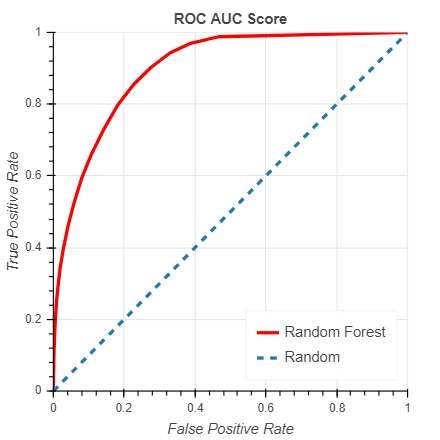
\includegraphics[scale=0.45]{random_forest_roc}
  \centering
  \caption{Random Forest ROC AUC curve}
  \label{fig:random_forest_roc}
\end{figure}

\begin{figure}
  \begin{tabular}{ll}
    \textbf{Feature}                          & \textbf{Importance} \\
    GENSTAT (Generation status)               & 0.062281 \\
    ETHDER (Ethnic origin)                    & 0.0573086 \\
    PR (Province, current)                    & 0.0523802 \\
    POBM (Mother's POB)                       & 0.048009 \\
    POB (Place of birth)                      & 0.0405777 \\
    POBF (Father's POB)                       & 0.0321791 \\
    VisMin (Visible minority status)          & 0.0253287 \\
    AGEGRP (Age)                              & 0.0240645 \\
    PR5 (Province, 5 years ago)               & 0.0239604 \\
    IMMCAT5 (Immigration admission category)  & 0.0232537
  \end{tabular}
  \caption{Random Forest feature importances}
  \label{fig:random_forest_importances}
\end{figure}

\begin{figure}
  \begin{tabular}{lllll}
                  & precision & recall      & f1-score  & support \\
  \textit{False}  & 0.93      & 0.68        & 0.79      & 76719 \\
  \textit{True}   & 0.37      & 0.80        & 0.51      & 18050 \\
  Total			      &           &             &           & 94769 \\
  Accuracy        & 0.71 \\
  ROC AUC Score	  & 0.82 \\\
  \end{tabular}
  \caption{Naive Bayes metrics}
  \label{fig:naive_bayes_metrics}
\end{figure}

\begin{figure}
  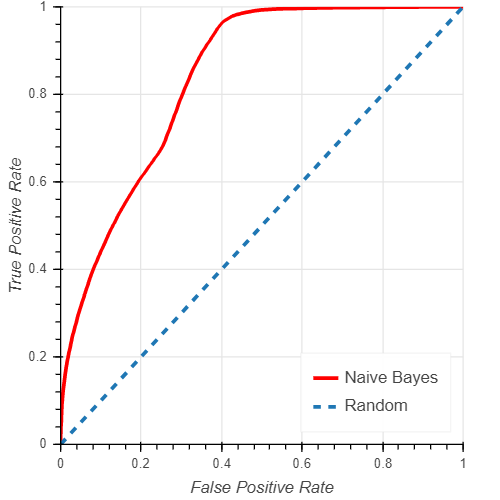
\includegraphics[scale=0.45]{naive_bayes_roc}
  \centering
  \caption{Naive Bayes ROC AUC curve}
  \label{fig:naive_bayes_roc}
\end{figure}


\section{Conclusion}
% @TODO fill in
In this paper, the performance of 3 different supervised learning techniques was compared when applied to the 2016 Canadian public census data by various metrics.

The results indicate that the Random Forest classifier outperformed the Decision Tree classifier and Naive Bayes classifier in general. The Random Forest and Decision Tree classifiers were quite proficient in detecting a lack of language shift, but were significantly less accurate in classifying a language shift. Contrasting this, the Naive Bayes classifier was better in detecting a language shift and was worse in detecting the lack of a language shift. Finally, the Decision Tree and Random Forest classifiers performed quite similarly, with the Random Forest classifier slightly outperforming the Decision Tree variant.


\subsection{Future Work}
% @TODO fill in
One aspect that could be improved on in future work is to tweak the hyper parameters for the classifiers via cross validation. For instance, setting different values for the max tree depth on the Decision Tree classifier, or setting different values for the number of trees in the Random Forest classifier. Modifying these values may result in a more accurate classifier.

Additionally, the 2016 Canadian Census data set contains mostly data indicating a lack of language shift. As a result, the classifiers learn mostly on these negative results, and it may impact the rates for positive results. The weights on the training data could be re-weighted to account for this, but further complications may arise when trying to maintain the data being representative of the Canadian public.

Furthermore, this analysis could be applied over multiple census years. In addition to increasing the amount of data available, adding a temporal dimension could add an interesting aspect to the classifiers, possibly taking historical events into account.

Adding a geographical dimension to the classifiers could identify more granular language shifts in Canadian provinces and territories. It would be interesting to apply the analysis on municipalities such as the City of Winnipeg as well. The Winnipeg open census data portal contains information on language spoken broken down by neighbourhood and ward.

Another interesting metric that could be determined in future work is the conditional probability of each category of each feature influencing the language shift category. For instance, \textit{scikit-learn}'s CategoricalNB classifier implementation contains a feature log prob attribute that returns a 2D array for each feature, which contains the logarithmic probability that each category of the feature influences the language shift category.

\section*{Acknowledgment}


The authors would like to thank the staff at the Elizabeth Dafoe library for giving direction on locating census microdata, and Dr. Carson Leung of the Databases and Data Mining Laboratory at the University of Manitoba for support of this project.




\bibliographystyle{IEEEtran}
\bibliography{bare_conf}

\end{document}


